%\section{A New Framework for On-Stack Replacement}
\section{A Flexible On-Stack Replacement Framework}

Modern language runtimes dynamically adapt the execution to the actual workload, maintaining different versions of the code generated with different, often speculative, optimizations. For this reason, they typically implement on-stack replacement mechanisms to dynamically transfer execution between them while a version of the method to optimize is still running.

Pioneered in the SELF language runtime in the early '90s~\cite{Holzle92}, OSR mechanisms have drawn considerable attention from the community of VM builders as the Java language became popular. OSR is nowadays used in a relevant number of virtual machines to implement optimization techniques such as profile-driven and deferred compilation, and can also be employed to support debugging of optimized code.

\noindent OSR can be a very powerful tool for implementing dynamic languages, for which most effective optimization decisions can typically be made only at run time, when critical information such as type and shape of objects becomes available. In this scenario, OSR becomes useful also to perform deoptimization, i.e., when the running code has been speculatively optimized and one of the assumptions does not hold anymore, the optimized function is interrupted and the execution continues in a safe version of the code.

\paragraph*{Contributions.} In this thesis, we propose a general-purpose, target-independent framework for OSR. Specific goals of our solution include:
\begin{itemize}[parsep=0pt]
\item The ability for a function reached via OSR to fire an OSR itself: this would allow switching from a base function $f$ to an optimized function $f'$, and later on to a further optimized version $f''$, and so on.
\item Supporting deoptimization, i.e., transitions from an optimized function to a less optimized function from which it was derived.
\item Supporting transitions at arbitrary program points, including those that would require adjusting the transferred program state to resume the execution in the OSR target function.
\item Supporting OSR targets either generated at run-time (e.g., using profiling information) or already known at compilation time.
\item Hiding from the front-end that generates the different function versions all the implementation details for handling OSR transitions between them.% at specific points.
\end{itemize}

\noindent We show the feasibility of our approach by implementing \osrkit, a prototype OSR library for the MCJIT just-in-time compiler of the LLVM compiler infrastructure.

\subsection{Approach}
\label{ss:osr-llvm-approach}

The key to generality and platform-independence in our approach is to express the OSR machinery entirely at intermediate representation (IR) level, without resorting to native-code manipulation or special compiler intrinsics.

\ifdefined\noauthorea
\begin{figure}[hb]
\vspace{4mm} % TODO remove this
\begin{center}
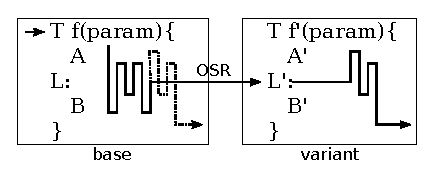
\includegraphics[width=0.6\textwidth]{figures/osr-dynamics/osr-dynamics.eps}
\caption{\protect\label{fig:osr-dynamics} On-stack replacement dynamics: control is transferred via OSR from a point \textsf{L} of a base function \textsf{f} to a point \textsf{L'} in a variant \textsf{f'} of \textsf{f}.}
\end{center}
\end{figure}
\fi

\noindent Consider the generic OSR scenario shown in \myfigure\ref{fig:osr-dynamics}. A base function \fbase\ is executed and it can either terminate normally (dashed lines), or an OSR event may transfer control to a variant \fvariant, which resumes the execution. The decision of whether an OSR should be fired at a given point \osrpoint\ of \fbase\ is based on an {\em OSR condition}. A typical example in JIT-based virtual machines is a profile counter reaching a certain hotness threshold, which indicates that \fbase\ has been executing for some time and is worth optimizing. Another example is a guard testing whether \fbase\ has become unsafe and execution needs to fall back to a safe version \fvariant. This scenario includes deoptimization of functions generated with aggressive speculative optimizations.

Several OSR implementations adjust the stack so that execution can continue in \fvariant\ with the current frame \cite{Chambers91, Chambers92, Holzle92, Suganuma06}. This requires manipulating the program state at machine-code level and is highly ABI- and compiler-dependent. A simpler approach, which we follow in this thesis, consists in creating a new frame every time an OSR is fired, essentially regarding an OSR transition as a function call~\cite{Lameed13,Pizlo14}. Our solution targets two general scenarios:
\begin{enumerate}[parsep=0pt]
 \item {\em resolved OSR}: \fvariant\ is known before executing \fbase\ as in the deoptimization example discussed above;
 \item {\em open OSR}: \fvariant\ is generated when the OSR is fired, supporting for instance deferred and profile-guided compilation strategies.
\end{enumerate}

\noindent In both cases, \fbase\ is instrumented before its execution to incorporate the OSR machinery. We call such OSR-instrumented version \fosrfrom.

In the resolved OSR scenario (see \myfigure\ref{fig:osr-resolved}), instrumentation consists of adding a check of the OSR condition and, if it is satisfied, a tail call that fires the OSR. The called function is an instrumented version of \fvariant, which we call \fosrto. We refer to \fosrto\ as the {\em continuation function} for an OSR transition. The assumption is that \fosrto\ produces the same side-effects and return value that one would obtain from \fbase\ if no OSR was performed. Differently from \fvariant, \fosrto\ takes as input all live variables of \fbase\ at \osrpoint, executes an optional {\em compensation code} to fix the computation state ({\tt comp\_code}), and then jumps to a point \textsf{L'} from which execution can continue.

\ifdefined\noauthorea
\begin{figure}[b]
\begin{center}
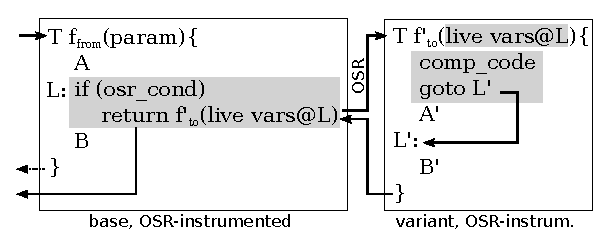
\includegraphics[width=0.7\textwidth]{figures/osr-resolved/osr-resolved.eps}
\caption{\protect\label{fig:osr-resolved} Resolved OSR scenario.}
\end{center}
\end{figure}
\fi

%Compensation code adds flexibility to our framework, as it extends the range of points where OSR transitions can be fired. In fact, the OSR practice often makes the conservative assumption that execution can always continue with the very same program state as the base function. This assumption can however be restrictive, as it may reduce the number of program locations eligible for OSR (i.e., one has to wait to a point where the states would correspond). Our solution provides a front-end with means to encode a compensation code, tailored to the specific optimizations involved between two function versions, that is needed to adjust the program state and perform an OSR at an arbitrary given location.

Compensation code adds flexibility to our framework, as it extends the range of points where OSR transitions can be fired. In fact, the OSR practice often makes the conservative assumption that execution can always continue with the very same program state as the base function. %This assumption may however reduce the number of OSR opportunities, e.g., one has to wait to a point where the states would correspond.
This assumption can however be restrictive, as it may reduce the number of program locations eligible for OSR (i.e., one has to wait to a point where the states would realign). Our solution provides a front-end with means to encode a glue code, tailored to the specific optimizations involved between two function versions, to adjust the program state and perform an OSR transition. This code can be used, for instance, to modify the heap, or to reconstruct values for variables that are live at \textsf{L'} but not at \textsf{L}.

The open OSR scenario is similar, with one main difference (see \myfigure\ref{fig:osr-open}): instead of calling \fosrto\ directly, \fosrfrom\ calls a stub function \fstub, which first creates \fosrto\ and then calls it. Function \fosrto\ is generated by a function {\tt gen} that takes the base function \fbase\ and the OSR point \osrpoint\ as input. The reason for having a stub in the open OSR scenario, rather than directly instrumenting \fbase\ with the code generation machinery, is to minimize the extra code injected into \fbase. Indeed, instrumentation may interfere with optimizations, e.g., by increasing register pressure and altering code layout and instruction cache behavior.

%\mynote{JIT compilation?}

\ifdefined\noauthorea
\begin{figure}[t]
\begin{center}
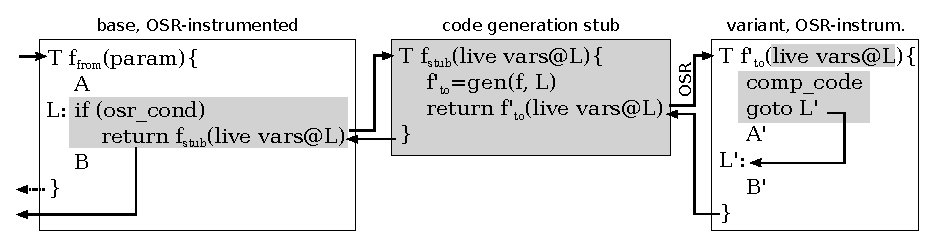
\includegraphics[width=1.0\textwidth]{figures/osr-open/osr-open.eps}
\caption{\protect\label{fig:osr-open} Open OSR scenario.





}
\end{center}
\end{figure}
\fi

%\subsection{Implementing OSR in LLVM}
\subsection{LLVM Implementation}
\label{ss:osrkit-implementation}

The LLVM compiler infrastructure~\cite{Lattner04} provides a Just-In-Time compiler called MCJIT that is currently being used for generating optimized code at run-time in virtual machines for dynamic languages. MCJIT is employed in both industrial and research projects, including WebKit's JavaScript engine, the open-source Python implementation Pyston, the Rubinius project for Ruby, Julia for high-performance technical computing, McVM for MATLAB, CXXR/Rho for the R language, Terra for Lua, and the Pure functional programming language. The MCJIT compiler shares the same optimization pipeline with LLVM front-ends for static languages such as \clang, and it provides dynamic features such as native code loading and linking, as well as a customizable memory manager for code and data sections.

Currently VM builders using MCJIT are required to have a deep knowledge of the internals of LLVM in order to mimic an OSR mechanism. In particular, they can rely on two experimental intrinsics, {\em Stackmap} and {\em Patchpoint}, to inspect the details of the compiled code generated by the back-end and to patch it manually with a sequence of assembly instructions. A {\em Stackmap} is used to record the run-time location (i.e., register, stack offset or constant) for a set of variables (e.g., the set of live variables) at a given IR instruction. The intrinsic generates no code in place\footnote{Although a front-end can ask LLVM to pad the function with a number of NOP instructions to prevent overwriting program text or data outside its boundaries during the run-time patching.}, as the back-end emits its data into a designated section in the object code. A Stackmap allows the runtime to disruptively patch the original code in response to an event triggered from outside, thus executing a new code sequence when the location for the original IR instruction is reached. A {\em Patchpoint} instead creates a function call to a target typically not known at compile time, and implies a StackMap generation to track the run-time location for the set of variables given as argument. A Patchpoint reserves space for injecting new code (e.g., to update the target of the call), so that the other instructions in the function are preserved. An example application of the Patchpoint intrinsic is the implementation~\cite{Pizlo14} of an inline caching mechanism~\cite{Deutsch84} for polymorphic method dispatch in WebKit's JavaScript engine. Both intrinsics are currently marked as experimental in LLVM, and are treated along the optimization pipeline as instructions that can potentially read and write all memory\footnote{A {\tt store} instruction clearly cannot be moved across a Stackmap, but also a {\tt load} must be handled conservatively (i.e., cannot be hoisted above it) as it might trigger an exception.}.

%\mynote{Dire della differenza con GC Stack Map?}

%In particular, a Stackmap records the location of live values at a particular instruction address and during the compilation it is emitted into the object code within a designated section; a Patchpoint instead allows to reserve space at an instruction address for run-time patching and can be used to implement an inline caching mechanism~\cite{Pizlo14, Deutsch84}.

%avoiding low-lever tampering with stack frames can more easily preserve ABI calling conventions

We prototyped our idea of flexible OSR infrastructure working entirely at IR level in a library for MCJIT called \osrkit. \osrkit\ provides a number of useful abstractions that include open and resolved OSR instrumentation of IR base functions without breaking the SSA (Static Single Assignment) form~\cite{Cytron91}, liveness analysis, generation of OSR continuation functions, and mapping of LLVM values between different function versions along with an interface for compensation code generation.

We also implemented a proof-of-concept VM called \tinyvm\ that provides an interactive environment for LLVM IR manipulation, JIT compilation, and benchmarking. All of our code is publicly available and has been endorsed by the joint Artifact Evaluation process of CGO-PPoPP 2016.

\subsubsection*{A Running Example}
We present our OSR embodiment for LLVM through a simple running example that illustrates a profile-driven optimization scenario. We start from a simple base function ({\tt isord}) that checks whether an array of numbers is ordered according to some criterion specified by a comparator (see \myfigure\ref{fig:osr-isord}). Our goal is to instrument {\tt isord} so that, whenever the number of loop iterations exceeds a certain threshold, control is dynamically diverted to a faster version generated on the fly by inlining the comparator. The IR code shown in this section has been generated with \clang\ and later instrumented with \osrkit\ inside \tinyvm. Virtual register names and basic block labels have been refactored for the sake of readability.

\ifdefined\noauthorea
\begin{figure}[t]
\begin{center}
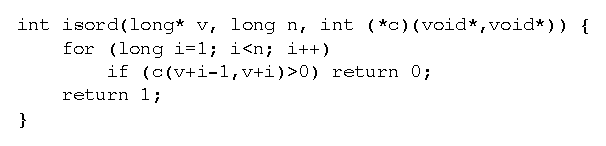
\includegraphics[width=0.66\textwidth]{figures/osr-isord/osr-isord.eps}
\caption{\protect\label{fig:osr-isord} Example for OSR instrumentation in LLVM.
}
\end{center}
\end{figure}
\fi

\ifdefined\noauthorea
\begin{figure}[!ht]
\begin{center}
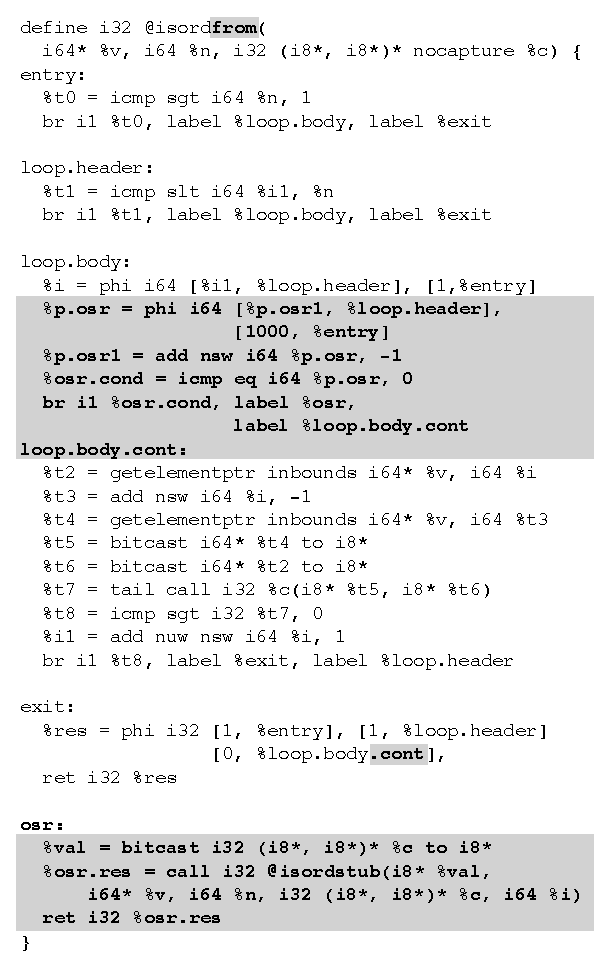
\includegraphics[width=0.66\textwidth]{figures/osr-isordfrom/osr-isordfrom.eps}
\caption{\protect\label{fig:osr-isordfrom} LLVM IR version of base function {\tt isord} (\myfigure\ref{fig:osr-isord}) instrumented for open OSR. Additions resulting from the instrumentation are in grey. The OSR is fired at the beginning of the loop body after 1000 iterations, i.e., when the counter reaches 0.

}
\end{center}
\vspace{-2mm}
\end{figure}
\fi

\paragraph*{IR Instrumentation.}
To defer the compilation of the continuation function until the comparator is known at run time, we used \osrkit\ to instrument {\tt isord} with an open OSR point at the beginning of the loop body, as shown in \myfigure\ref{fig:osr-isordfrom}. Portions added to the original code by OSR instrumentation are highlighted in grey.

\noindent New instructions are placed at the beginning of the loop body to increment a hotness counter {\tt p.osr} and jump to an OSR-firing block if the counter reaches the threshold (1000 iterations in this example). The OSR block contains a tail call to the target generation stub, which receives as parameters the four live variables at the OSR point ({\tt v}, {\tt n}, {\tt c}, {\tt i}). \osrkit\ allows the stub to receive the run-time value {\tt val} of an IR object that can be used to produce the continuation function -- in our example, the pointer to the comparator function to be inlined. The stub (shown in \myfigure\ref{fig:osr-isordstub}) calls a code generator that:
\begin{enumerate}[parsep=0pt,itemsep=3pt]
 \item builds an optimized version of {\tt isord} by inlining the comparator, and
 \item uses it to create the continuation function {\tt isordto} shown in \myfigure\ref{fig:osr-isordto}.
\end{enumerate}

\noindent The stub passes to the code generator four parameters:
\begin{enumerate}[parsep=0pt,itemsep=3pt]
 \item a pointer to the {\tt isord} IR code;
 \item a pointer to the basic block in {\tt isord} from which the OSR is fired;
 \item a pointer to a user-defined object to support code generation in MCJIT;
 \item the stub's {\tt val} parameter.
\end{enumerate}

\noindent The first three parameters are provided by the front-end and hard-wired by \osrkit. In particular, the third parameter is a handle to the environment for code generation (e.g., in our dynamic inliner the object contains pointers to the MCJIT engine and to a map between addresses of compiled functions and their IR counterparts). The stub terminates with a tail call to {\tt isordto}.

\ifdefined\noauthorea
\begin{figure}[ht]
\begin{center}
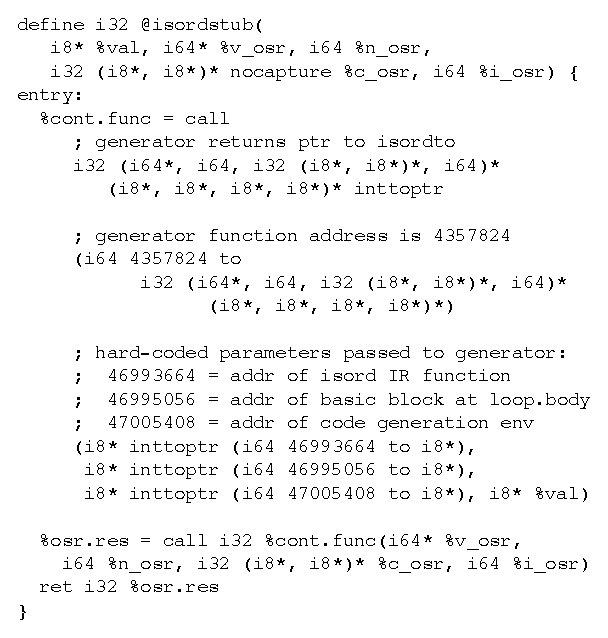
\includegraphics[width=0.66\textwidth]{figures/osr-isordstub/osr-isordstub.eps}
\caption{\protect\label{fig:osr-isordstub} IR stub that generates the continuation function when an open OSR is fired by {\tt isordfrom} (\myfigure\ref{fig:osr-isordfrom}).
}
\end{center}
\end{figure}
\fi

\noindent To generate the continuation function (shown in \myfigure\ref{fig:osr-isordto}) from the optimized version created by the inliner, \osrkit\ replaces the function entry point, removes dead code, replaces live variables with the function parameters, and fixes $\phi$-nodes accordingly. As the OSR transition does not require modifications to the program state, the new entry point does not contain any compensation code. Preserving the SSA form while constructing the continuation function is a challenging task, as it might require inserting new $\phi$-nodes in the control-flow graph in addition to simply updating some of the existing ones as in this example. When generating a continuation function, we use a modified version of LLVM's {\tt SSAUpdater} component to account for the available values -- transferred as parameters or reconstructed in the OSR entrypoint -- of all the variables that are live at the OSR landing pad.

%\vspace{-4mm}

%Additions resulting from the IR instrumentation are in grey, while removals are struck-through.

\ifdefined\noauthorea
\begin{figure}[t]
\begin{center}
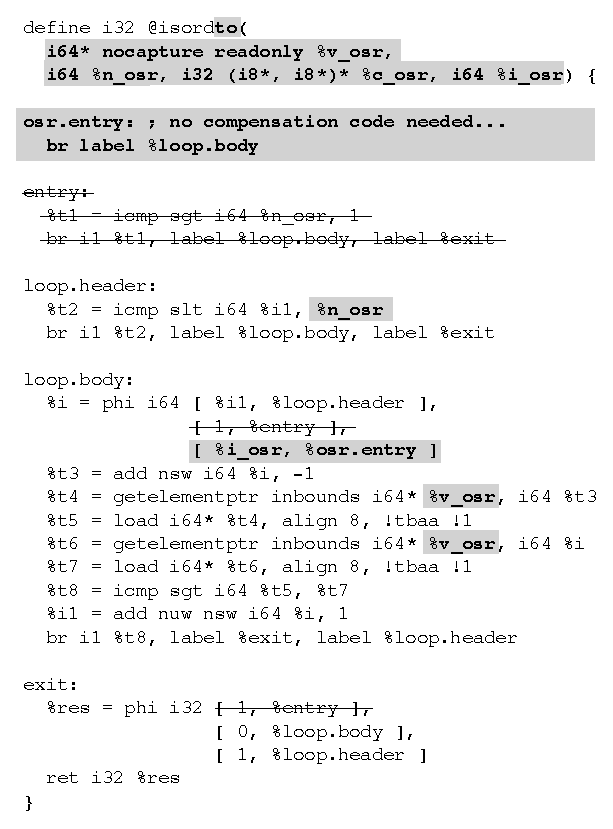
\includegraphics[width=0.66\columnwidth]{figures/osr-isordto/osr-isordto.eps}
\caption{\protect\label{fig:osr-isordto} Faster variant of {\tt isord} (\myfigure\ref{fig:osr-isord}) in LLVM IR with comparator inlining, instrumented as OSR continuation function. Instrumentation additions are in grey. The original function entry block is unreachable after instrumentation and is eliminated (struck-through code fragments).
}
\end{center}
\end{figure}
\fi

\ifdefined\noauthorea
\begin{figure}[t]
\begin{center}
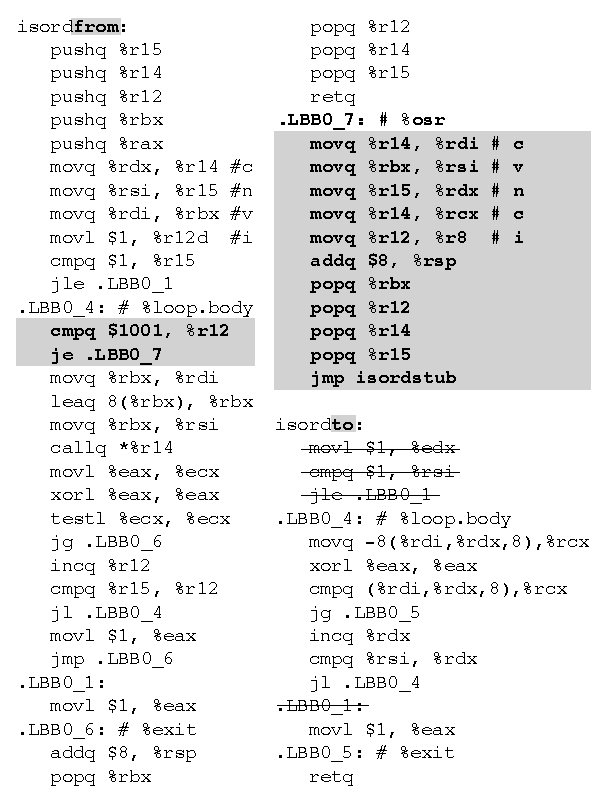
\includegraphics[width=0.66\columnwidth]{figures/osr-isord-x86_64/osr-isord-x86_64.eps}
\caption{\protect\label{fig:osr-isordx86_64} OSR-instrumented functions {\tt isordfrom} (base) and {\tt isordto} (faster continuation) after IR-to-x86-64 lowering in LLVM. %For the sake of comparison with the native code that would be generated for the original non-OSR versions,
Additions resulting from the IR instrumentation are in grey, while removals are struck-through.
}
\end{center}
\end{figure}
\fi

\paragraph*{x86-64 Lowering.}

%The final step to be performed before execution is native code generation. 
\myfigure\ref{fig:osr-isordx86_64} shows the x86-64 code generated by the LLVM back-end for {\tt isordfrom} and {\tt isordto}. For the sake of comparison with the native code that would be generated for the original non-OSR versions, additions resulting from the IR instrumentation are in grey, while removals are struck-through.

Notice that the OSR intrusiveness in {\tt isordfrom} is minimal, consisting of just two assembly instructions with register and immediate operands. As a result of induction variable canonicalization in the LLVM back-end, loop index {\tt i} and hotness counter {\tt p.osr} are fused in register {\tt\%r12}. We also note that tail call optimization is applied in the OSR-firing block, resulting in no stack growth during an OSR.

\noindent The continuation function {\tt isordto} is identical to the specialized version of {\tt isord} with inlined comparator, except that the loop index is passed as a parameter in {\tt \%rdx} and no %loop pre-header 
preamble is needed since OSR jumps directly in the loop body.

\subsection{Discussion}
Instrumenting functions for OSR at a higher level than machine code yields several benefits: 
\begin{enumerate}[parsep=0pt]
\item {\em Platform independence}: the OSR instrumentation code is lowered to native code by the compiler back-end, which handles the details of the target ABI. 
\item {\em Global optimizations}: lowering OSR instrumentation code along with application code can generate faster code than local binary instrumentation. For instance, dead code elimination can suppress from \fosrto\ portions of code that would no longer be needed when jumping to the landing pad \textsf{L'}, producing smaller code and enabling better register allocation and instruction scheduling.
\item {\em Debugging and Profiling}: preserving ABI conventions in the native code versions of \fosrfrom, \fstub, and \fosrto\ helps debuggers and profilers to more precisely locate the current execution context and collect more informative data.
%avoiding low-lever tampering with stack frames can more easily preserve ABI calling conventions
\item {\em Abstraction}: being entirely encoded using high-level language constructs (assignments, conditionals, function calls), the approach is amenable to a clean instrumentation API that abstracts the OSR implementation details, allowing a front-end to focus on where to insert OSR points independently of the final target architecture.
%by analyzing code at an intermediate representation level.
\end{enumerate}

\noindent A natural question is whether encoding OSR at a higher level of abstraction can result in poorer performance than binary code approaches. Our solution relies on the compiler's compilation pipeline to generate the most efficient native code for \fosrfrom\ and \fosrto. We provide performance numbers in \mysection\ref{se:eval-osrkit} by measuring the overhead of \osrkit\ on classic benchmarks.

To the best of our knowledge, our framework is the first to support OSR point insertion at arbitrary locations in the code. There was considerable implementation and experimentation effort to show its feasibility. In order to enable OSR at any program point, two engineering aspects are involved: manipulating the code of an optimized function to generate a continuation function -- a task that can be daunting as the SSA form must be preserved -- and providing a front-end with a clean interface to specify glue code that might be required to perform a transition. Encoding compensation code with our API is currently delegated to the front-end. In \mysection\ref{ss:osr-mapping} we will provide an algorithm to automatically build it for a number of common compiler optimizations.

A possible scenario in which supporting OSR at arbitrary locations can be particularly useful is the implementation a flexible deoptimization mechanism in the presence of aggressive speculative optimizations. In general, it might be necessary to have a deoptimization point in the middle of a heavily optimized code fragment. Our framework provides VM builders with means to perform deoptimization without requiring a fallback to an interpreter. Also, by supporting both open and resolved OSR points we allow them to explore the trade-off between the latency from creating continuation functions on-the-fly and the code bloat from doing it ahead-of-time.

In the case study presented \mysection\ref{se:CS-matlab} we explore the end-to-end utility of \osrkit\ to tackle performance problems deriving from the use of a higher-order construct in the MATLAB language. The ability of \osrkit\ to insert OSR points at arbitrary locations allows us to capture uses of this construct and to trigger an OSR transition to a much more type-specialized version of the code.

%In general, control flow might leave a function in the middle of a heavily optimized fragment (e.g., a loop body), execute a glue code to adjust the state when needed, and continue in a different, safe version of the same function. We remark that our framework is optimization-agnostic, and supporting both open and resolved OSR points provides VM builders with different trade-offs between code bloat and latency from JIT compilation.
%\mynote{VMs do it already, so... we should rephrase this paragraph!}

 %as it stricly depends on the optimizations it performs

%In Section\missing\ we present a case study in the McVM runtime for the MATLAB language, showing \missing.

\subsection{Comparison with Related Work}
\label{ss:osr-llvm-related}

\paragraph*{Early Approaches.} OSR has been pioneered in the SELF programming language implementations~\cite{Holzle92} to enable source-level debugging of optimized code, which requires deoptimizing the code back to the original version. To reconstruct the source-level state, the compiler generates {\em scope descriptors} recording locations or values of arguments and locals. Execution can be interrupted only at certain interrupt points where its state is guaranteed to be consistent (i.e., method prologues and backward branches in loops), allowing optimizations between interrupt points. SELF also implements a deferred compilation mechanism~\cite{Chambers91} for branches that are unlikely to occur at run-time: the system generates a stub that invokes the compiler to generate a code object that can reuse the stack frame of the original code. Open OSR points proposed in this thesis can be used to implement deferred compilation at any basic block in a similar manner.

\paragraph*{Java Virtual Machines.} The success of the Java language has drawn more attention to the design and implementation of OSR techniques, as bytecode interpreters began to work along with JIT compilers. In the high-performance HotSpot Server JVM~\cite{Paleczny01} performance-critical methods are identified using method-entry and backward-branches counters; when the OSR threshold is reached, the runtime transfers the execution from the interpreter frame to an OSR frame and thus to compiled code. Deoptimization is performed when class loading invalidates inlining or other optimization decisions: execution is rolled forward to a safe point, at which the native frame is converted into an interpreter frame.

%Whaley~\cite{Whaley01} proposes a technique to identify intra-method code regions that are rarely executed, and thus compile and optimize the code without these regions. A rare block is replaced by a stub that transfers the control to the interpreter, while a glue routine reconstructs the state from the interpreter starting from a table storing the location, in registers or memory, of each variable in the original bytecode.

The Jikes RVM uses an OSR mechanism~\cite{Fink03} that extracts a scope descriptor from a thread suspended at a method's entrypoint or backward branch, creates specialized code to setup the stack frame for the optimized compiled code and resumes the execution at the desired program counter.
OSR is used as part of an automatic, online, profile-driven deferred compilation mechanism. The specialized code used in Jikes RVM is equivalent to the continuation function generated by our framework. % discuss constants being hard-wired in it? (partial evaluation)
A more general approach has then been proposed in~\cite{Soman06}, with the OSR implementation decoupled from program code to ease more aggressive specializations triggered by events external to the executing code (e.g., class loading, exception conditions). Execution state information is maintained in a variable map - a per-method list of thread-switch points and associated live bytecode variables - that is incrementally updated across a number of basic compiler optimizations. % a wide range of

In the Graal VM - a modified version of HotSpot centered on the principle of speculative optimizations - execution falls back to the interpreter during deoptimization, while a runtime function restores the stack frames in the interpreter using the metadata associated with the deoptimization point~\cite{Duboscq13,Wurthinger13,Duboscq14}.

\paragraph*{Prospect.} Prospect~\cite{Susskraut10} is an LLVM-based framework for parallelizing a sequential application. The IR is instrumented through two LLVM passes to enable switching at run-time between a slow and a fast variant of the code, which are both compiled statically. Helper methods are used to save and eventually restore registers, while stack-local variables are put on a separate \alloca\ stack rather than on the stack frame so that the two variants result into similar and thus interchangeable stack layouts.
%Speculative variables~\cite{Susskraut09} are introduced when the slow variant needs to track state (e.g., information for out-of-bound checks) that is missing in the fast variant.
Switching operations are performed by Prospect at user-specified checkpoints in the original code. Although both Prospect and \osrkit\ support switching execution between two variants of a function, they target different applications.

\paragraph*{McOSR.} McOSR~\cite{Lameed13} is a library for inserting open OSR points designed specifically for the legacy LLVM JIT, and encodes the OSR machinery entirely in IR as \osrkit\ does. When an OSR is fired, live variables are stored into a pool of globals allocated by the library. McOSR then invokes a user-defined method to transform \fbase\ into \fvariant\ and calls \fbase\ with empty parameters. The new entrypoint inserted by McOSR in \fbase\ checks a global flag to discriminate if the function is being invoked in an OSR transition or as a regular call: in the first case, the state is restored from the pool of global variables before jumping to the OSR landing pad.

\osrkit\ improves upon McOSR in a number of aspects. The presence of a new entrypoint has the potential to disrupt many optimizations: McOSR tries to mitigate this issue by promptly recompiling \fbase\ again once the execution is resumed and \fbase\ has returned, but only future invocations of \fbase\ would benefit from it. In contrast, \osrkit\ generates an optimized, dedicated OSR continuation function to resume the execution: lessons from the Jikes RVM~\cite{Fink03} suggest that our approach is likely to yield better performance. Also, we transfer live variables as arguments to the continuation function, possibly using registers, which is likely to be more efficient than spilling them to a pool of globals.
%variables maintained by the VM.
Due to the complexity in preserving the SSA form when updating the IR, McOSR allows the insertion of OSR points only at loop headers (in particular, those with exactly two predecessor blocks), while \osrkit\ can encode them at arbitrary program locations.

Notice also that \osrkit\ introduces a number of features that are absent from McOSR, including: support for compensation code and resolved OSR points; compatibility with MCJIT's design; support for maintaining multiple versions of the same function, which can be very useful in the presence of speculative optimizations and deoptimization.

\paragraph*{Other Related Work.}
Dynamic Software Updating (DSU) is a methodology for permitting programs to be updated while they run and is thus useful for systems that cannot afford to halt service. DSU techniques (e.g., ~\cite{Neamtiu06,Makris09}) are required to update all functions active on the call stack at the same time, so their code should be instrumented and data types wrapped to support future extensions. Albeit DSU and OSR both manipulate the stack to replace running functions, they target dissimilar applications, and the performance constraints they are subject to are different. 

In tracing JIT compilers deoptimization techniques are used to safely leave an optimized trace when a guard fails. SPUR~\cite{Bebenita10} is a trace-based JIT compiler for Microsoft's Common Intermediate Language (CIL) with three levels of JIT-ting plus a transfer-tail JIT used to bridge the execution from an instruction in a block generated at the second or third level to a safe point for deoptimization to the first JIT level. Deoptimization can thus happen without falling back to an interpreter; similarly, our approach enables VM builders to perform OSR transitions working at native-code level only.

In RPython, guards are implemented as a conditional jump to a trampoline that analyzes resume information for the guard and executes compensation code to leave the trace; resume data is compactly encoded by sharing parts of the data structure between subsequent guards~\cite{Schneider12}. A similar approach is used in LuaJIT, where sparse snapshots are taken to enable state restoration when leaving a trace~\cite{luajit}. For deoptimization purposes, it would be interesting to investigate whether, given a sequence of source instructions, a single continuation function could be created, by adding a dispatcher in its entry block that compensates the state according to the current source for the OSR.